\documentclass[11pt]{llncs}
\usepackage{preamble}

\begin{document}
\title{
Set Theory Class 2018 - 2019\\
Exercise Set 2}
\date{\today}
\author{Dionysis Zindros\\
    \email{dionyziz@di.uoa.gr}}
\institute{
National and Kapodistrian University of Athens}
\maketitle
\noindent
\makebox[\linewidth]{\small \today}

\thispagestyle{plain}

\section*{Exercise 1}
\begin{lemma}
  $\omega \not\in \omega$.
\end{lemma}
\begin{proof}
  Suppose for contradiction that $\omega = n$ for some $n \in \omega$. Then
  $n \in n$, which is a contradiction.
  \qed
\end{proof}

\begin{lemma}
  $\forall n \in \omega: \omega \not\in n$.
\end{lemma}
\begin{proof}
  Let $S = \{n \in \omega: \omega \not\in n\}$. We will show $S = \omega$.
  By induction. $0 \in S$, as $\omega \not\in \emptyset$. Suppose
  $\omega \not\in n$, and suppose for contradiction that
  $\omega \in n\cup\{n\}$. Then $\omega = n$, hence $\omega \in \omega$, which
  is a contradiction.
  \qed
\end{proof}

\begin{lemma}
  $\forall n \in \omega$, $n$ is not inductive.
\end{lemma}
\begin{proof}
  Suppose for contradiction $n$ were inductive. Then $\omega \subseteq n$, and
  so $n \in n$, which is a contradiction.
  \qed
\end{proof}

\begin{lemma}
  $\omega \cup \{\omega\} \not\in \omega$.
\end{lemma}
\begin{proof}
  Suppose for contradiction that $\omega \cup \{\omega\} \in \omega$. Then
  $\omega \cup \{\omega\} = n$ for some $n \in \omega$. Then $\omega \in n$,
  which is a contradiction.
  \qed
\end{proof}

\begin{lemma}
  $\omega \cup \{\omega\}$ is transitive.
\end{lemma}
\begin{proof}
  We already know that $\omega$ is transitive. To show that
  $\omega \cup \{\omega\}$ is transitive, it suffices to show that transitivity
  holds for the extra element, $\omega$. Indeed
  $\forall n \in \omega: n \in \omega$, and hence
  $n \in \omega \cup \{\omega\}$.
  \qed
\end{proof}

\begin{lemma}
  $\omega \cup \{\omega\}$ is not inductive.
\end{lemma}
\begin{proof}
  Suppose for contradiction that $S = \omega \cup \{\omega\}$ were inductive.
  Then $\omega \in S$ and hence $\omega \cup \{\omega\} \in S$, so $S \in S$.
  Hence either $S \in \omega$ or $S \in \{\omega\}$. In the first case, by
  virtue of $S$ being inductive,
  $\omega \in \omega$. In the second case, $S = \omega$, so
  $\omega \cup \{\omega\} = \omega$ hence again we have $\omega \in \omega$.
  This is a contradiction.
  \qed
\end{proof}

\section*{Exercise 2}
\begin{lemma}
  $\mathcal{P}(\omega) \not\in \omega$.
\end{lemma}
\begin{proof}
  Suppose for contradiction that $\mathcal{P}(\omega) \in \omega$.
  Then $\mathcal{P}(\omega) = n$ for some $n \in \omega$. But
  $\omega \in \mathcal{P}(\omega)$, so
  $\omega \in n$, which is a contradiction.
  \qed
\end{proof}

\begin{lemma}
  $\mathcal{P}(\omega)$ is not inductive.
\end{lemma}
\begin{proof}
  Suppose for contradiction that $\mathcal{P}(\omega)$ were inductive.
  $\omega \in \mathcal{P}(\omega)$, so
  $\omega \cup \{\omega\} \in \mathcal{P}(\omega)$. Therefore
  $\omega \cup \{\omega\} \subseteq \omega$ and $\omega \in \omega$, which is
  a contradiction.
  \qed
\end{proof}

\begin{lemma}
  $\omega \subseteq \mathcal{P}(\omega)$.
\end{lemma}
\begin{proof}
  Let $S = \{n \in \omega: n \in \mathcal{P}(\omega)\}$. We will show that
  $S = \omega$. By induction. As $\mathcal{P}(\omega)$ is a power set, we have
  that $\emptyset \in \mathcal{P}(\omega)$. Suppose $n \in \mathcal{P}(\omega)$,
  so $n \subseteq \omega$. But also $n \in \omega$, therefore
  $n \cup \{n\} \subseteq \omega$, which places
  $n \cup \{n\} \in \mathcal{P}(\omega)$.
  \qed
\end{proof}

\begin{lemma}
  $\mathcal{P}(\omega) \setminus \omega \neq \emptyset$.
\end{lemma}
\begin{proof}
  By counter-example. Clearly, $\omega \in \mathcal{P}(\omega)$, but
  $\omega \not\in \omega$.
  \qed
\end{proof}

Counter-examples are plenty. Another is the set $\{2\}$, which is in
$\mathcal{P}(\omega)$, but not in $\omega$, as every natural number
$k \in \omega$ has the property that, if it were to include a certain number
$n$, it must then also contain all of its preceding numbers $m < n$.

\section*{Exercise 3}
\begin{lemma}\label{lem:transitivity-equiv}
  Let $X$ be a set. The following statements are equivalent:
  \begin{enumerate}
    \item $X$ is transitive \label{item:transitivity-equiv-1}
    \item $X \subseteq \mathcal{P}(X)$ \label{item:transitivity-equiv-2}
    \item $\bigcup X \subseteq X$ \label{item:transitivity-equiv-3}
  \end{enumerate}
\end{lemma}
\begin{proof}
  \item{(\ref{item:transitivity-equiv-1} $\rightarrow$ \ref{item:transitivity-equiv-2})}
  Let arbitrary $a \in X$. We will show that $a \in \mathcal{P}(X)$.
  It suffices to show that $a \subseteq X$. Let arbitrary $b \in a$.
  We will show that $b \in X$. But $b \in a \in X$. From transitivity, $b \in X$.

  \item{(\ref{item:transitivity-equiv-2} $\rightarrow$ \ref{item:transitivity-equiv-3})}
  Let arbitrary $b \in \bigcup X$. We will show that $b \in X$.
  There exists some $a \in X$ such that $b \in a \in X$. From $X \subseteq \mathcal{P}(X)$ we get
  $a \in \mathcal{P}(X)$, so $a \subseteq X$. Therefore, $b \in X$.

  \item{(\ref{item:transitivity-equiv-3} $\rightarrow$ \ref{item:transitivity-equiv-1})}
  Let $b \in a \in X$. We will show that $b \in X$. $b \in \bigcup X$. From
  $\bigcup X \subseteq X$ we obtain $b \in X$.
  \qed
\end{proof}

\section*{Exercise 4}
\begin{lemma}
  Let $X$ be a transitive set. Then $\bigcup X$ is transitive.
\end{lemma}
\begin{proof}
  Let $b \in a \in \bigcup X$. We will show that $b \in \bigcup X$.
  There exists some $c$ such that $a \in c \in X$. From the transitivity of $X$,
  $a \in X$, so $b \in \bigcup X$.
  \qed
\end{proof}

The converse is not true. For example, consider the set
$X = \{\{\emptyset\}\}$. Then $\bigcup X = \{\emptyset\}$ is vacuously
transitive, but $X$ is not. This same example illustrates that if all the
elements of a set $X$ are transitive, this is not sufficient for $X$ itself
to be transitive. The converse is also false; if a set $X$ is transitive, not
all of its elements are necessarily transitive. For example,
$\{\{\{\emptyset\}\}, \{\emptyset\}, \emptyset\}$ is transitive, but
its element $\{\{\emptyset\}\}$ is not. However, if all elements of a set are
transitive, then its union is also transitive, as the following lemma
illustrates.

\begin{lemma}
  Let $X$ be a set such that for all $a \in X$, $a$ is transitive.
  Then $\bigcup X$ is transitive.
\end{lemma}
\begin{proof}
  Consider some $b \in a \in \bigcup X$. We will show that $b \in \bigcup X$.
  There exists some $c \in X$ such that $a \in c$. As an element of $X$, $c$ is
  transitive, hence $b \in c$, and so $b \in \bigcup X$.
  \qed
\end{proof}

\begin{lemma}
  Let $X$ be a set. $X$ is transitive iff $\mathcal{P}(X)$ is transitive.
\end{lemma}
\begin{proof}
  \item{($\rightarrow$)}
  Let $b \in a \in \mathcal{P}(X)$. We will prove that $b \in \mathcal{P}(X)$.
  $a \subseteq X$. $X$ is transitive, so apply
  Lemma~\ref{lem:transitivity-equiv} to obtain
  $X \subseteq \mathcal{P}(X)$. Hence, $a \subseteq \mathcal{P}(X)$ and so
  $b \in \mathcal{P}(X)$.

  \item{($\leftarrow$)}
  $\mathcal{P}(X)$ is transitive, so apply Lemma~\ref{lem:transitivity-equiv}
  to obtain $\bigcup\mathcal{P}(X) \subseteq \mathcal{P}(X)$.
  But $X = \bigcup\mathcal{P}(X)$, so $X \subseteq \mathcal{P}(X)$, which,
  by Lemma~\ref{lem:transitivity-equiv} shows that $X$ is transitive.
  \qed
\end{proof}

\section*{Exercise 5}
\begin{lemma}
  The set $X = \{n \in \omega: n \neq 0 \rightarrow \exists m: n = m^+\}$
  is inductive.
\end{lemma}
\begin{proof}
  $0 \in X$ because the premise is false.
  Suppose $m \in X$. We will show that $n = m^+ \in X$.
  It suffices to show that there exists some $m'$ such that $n = m'^+$.
  Letting $m' = m$, we arrive at the conclusion.
  \qed
\end{proof}

\section*{Exercise 6}
\begin{lemma}\label{lem:next-less}
  Let $m, n \in \omega$. Then
  $m < n \leftrightarrow m^+ \leq n$
\end{lemma}
\begin{proof}
  \item{($\rightarrow$)}
  $m < n$ means that both $m \subset n$ and $m \in n$.
  Therefore $m \cup \{m\} \subseteq n$, so $m^+ \leq n$.
  \item{($\leftarrow$)}
  If $m^+ = n$, then $m \cup \{m\} = n$ and so $m \subset n$, as $m \not\in m$.
  If $m^+ \neq n$, then $m^+ < n$. But $m < m^+$, so, by transitivity, $m < n$.
  \qed
\end{proof}

\begin{lemma}\label{lem:less-than-homo}
  Let $m, n \in \omega$. Then
  $m < n \leftrightarrow m^+ < n^+$
\end{lemma}
\begin{proof}
  \item{($\rightarrow$)}
  By Lemma~\ref{lem:next-less}, $m^+ \leq n$. Therefore $m^+ \subseteq n$.
  If $n \in m^+$, then $n \in n$, so we conclude that $n \not\in m^+$.
  Hence $m^+ \subset n \cup \{n\}$ and $m^+ < n^+$.

  \item{($\leftarrow)$}
  $m^+ < n^+$ means that $m \cup \{m\} \subseteq n \cup \{n\}$.
  Suppose for contradiction that $n \in m$. Then, by transitivity,
  $n \subseteq m$ and
  $n \cup \{n\} \subseteq m$, so $n \cup \{n\} \subseteq m \cup \{m\}$.
  Then $m^+ = n^+$, which is a contradiction, as $m^+ < n^+$.
  Hence, $n \not\in m$. Therefore $m \cup \{m\} \subseteq n$, so $m^+ \leq n$.
  By Lemma~\ref{lem:next-less} $m < n$.
  \qed
\end{proof}

\begin{lemma}\label{lem:less-right-next}
  Let $m, n \in \omega$. Then
  $m < n^+ \leftrightarrow m \leq n$
\end{lemma}
\begin{proof}
  By induction on $m$ we will show that for all $m$ the following holds:
  $\forall n \in \omega: m < n^+ \leftrightarrow m \leq n$.
  For $m = 0$ it holds, as both sides are always true. Suppose
  \begin{equation}\label{eq:less-than-next-ind1}
    \forall n \in \omega: m < n^+ \leftrightarrow m \leq n
  \end{equation}
  We will show that
  $\forall n \in \omega: m^+ < n^+ \leftrightarrow m^+ \leq n$.
  Let arbitrary $n \in \omega$. If $n = 0$ we are done, so suppose $n = k^+$.

  \item{($\rightarrow)$}
  Assume $m^+ < n^+$. Then by Lemma~\ref{lem:less-than-homo} we have
  $m < n$. By Equation~\ref{eq:less-than-next-ind1} we get $m \leq k$.
  If $m = k$ then $m^+ = n$. Otherwise, $m < k$.
  By Lemma~\ref{lem:less-than-homo} we obtain $m^+ < n$. In any case,
  $m^+ \leq n$.

  \item{($\leftarrow$)}
  Assume $m^+ \leq n$. If $m^+ = n$ then $m = k$. In that case, $m < n$
  and by Lemma~\ref{lem:less-than-homo} $m^+ < n^+$.
  If $m^+ < n$ then $n < n^+$ and
  therefore by transitivity of ``$<$'', $m^+ < n^+$.
  \qed
\end{proof}

\begin{lemma}
  Let $m, n \in \omega$. Then
  $m \leq n^+ \leftrightarrow (m \leq n \lor m = n^+)$.
\end{lemma}
\begin{proof}
  \item{($\rightarrow$)}
  If $m = n^+$ we are done. Let $m < n^+$. By Lemma~\ref{lem:less-right-next},
  $m \leq n$ and we are done.

  \item({$\leftarrow$})
  If $m \leq n$ then $n \leq n^+$ and by transitivity of ``$\leq$'' we have
  $m \leq n^+$. If $m = n^+$ then $m \leq n^+$.
  \qed
\end{proof}

\section*{Exercise 7}
\begin{lemma}
  $\forall m, n, k \in \omega: (m + n)k = mk + nk$.
\end{lemma}
\begin{proof}
  By induction on $k$. For $k = 0$: $(m + n)0 = m + n = m0 + n0$.
  Suppose $(m + n)k = mk + nk$. Then
  $(m + n)k^+ = (m + n)k + (m + n) = (mk + nk) + (m + n)$.
  But $mk^+ + nk^+ = mk + m + nk + n = (mk + nk) + (m + n)$.
  \qed
\end{proof}

\begin{lemma}
  $\forall m \in \omega: 0m = 0$.
\end{lemma}
\begin{proof}
  By induction on $m$. For $m = 0$: $0 \cdot 0 = 0$. Suppose $0m = 0$. Then
  $0m^+ = 0m + 0 = 0m = 0$.
  \qed
\end{proof}

\begin{lemma}
  $\forall m \in \omega: 1m = m$.
\end{lemma}
\begin{proof}
  By induction on $m$. For $m = 0$: $1 \cdot 0 = 0$. Suppose $1m = m$. Then
  $1m^+ = 1m + 1 = m + 1 = m^+$.
  \qed
\end{proof}

\begin{lemma}
  $m^+ = m + 1$.
\end{lemma}
\begin{proof}
  By induction on $m$. For $m = 0$, $0^+ = 1 = 0 + 1$.
  Suppose $m^+ = m + 1$. $m^{++} = (m + 1)^+$. By commutativity of ``$+$'' we
  have $(m + 1)^+ = (1 + m)^+ = 1 + m^+ = m^+ + 1$.
  \qed
\end{proof}

\begin{lemma}
  Multiplication is commutative.
\end{lemma}
\begin{proof}
  We will prove $\forall m \in \omega: \forall n \in \omega: mn = nm$.
  By induction on $m$. For $m = 0$, for all $n$, $0n = 0n = 0$.
  Suppose $\forall n \in \omega: mn = nm$ and let arbitrary $n \in \omega$.
  It suffices to show that $m^+n = nm^+$.
  $m^+n = (m + 1)n = mn + 1n = mn + n = nm + n$.
  But $nm^+ = nm + n$.
  \qed
\end{proof}

\begin{lemma}
  $\forall m, n, k \in \omega: k(m + n) = km + kn$.
\end{lemma}
\begin{proof}
  $k(m + n) = (m + n)k = mk + nk = km + kn = k(m + n)$.
  \qed
\end{proof}

\begin{lemma}\label{lem:addition-cancels}
  $\forall m, n, k \in \omega: k + m = k + n \rightarrow m = n$.
\end{lemma}
\begin{proof}
  By induction on $k$. For $k = 0$, suppose $0 + n = 0 + m$. Then
  $0 + n = n$ and $0 + m = m$, so $n = m$.
  Suppose $\forall m, n \in \omega: k + n = k + m \rightarrow m = n$.
  Let arbitrary $m, n \in \omega$ and suppose $k^+ + n = k^+ + m$.
  Then $n + k^+ = m + k^+$. But then $(n + k)^+ = (m + k)^+$ and so $n + k = m + k$.
  From the inductive hypothesis, $n = m$.
  \qed
\end{proof}

\section*{Exercise 8}
\begin{lemma}
  Multiplication is associative.
\end{lemma}
\begin{proof}
  We will show $\forall k, m, n \in \omega: k(mn) = (km)n$. By induction in $k$.
  For $k = 0$, $0(mn) = 0$ and $(0m)n = 0n = 0$.
  Suppose $\forall m, n \in \omega: k(mn) = (km)n$.
  Let arbitrary $m, n \in \omega$.
  \begin{align*}
  k^+(mn) &= (mn)k^+     &\text{(commutativity)}\\
          &= (mn)k + mn &\text{(multiplication definition)}\\
          &= k(mn) + mn &\text{(commutativity)}\\
          &= (km)n + mn &\text{(inductive hypothesis)}
  \end{align*}
  \begin{align*}
  (k^+m)n &= (mk^+)n     &\text{(commutativity)}\\
          &= (mk + m)n  &\text{(multiplication definition)}\\
          &= (mk)n + mn &\text{(distributivity)}\\
          &= (km)n + mn &\text{(commutativity)}
  \end{align*}
  \qed
\end{proof}

\begin{lemma}
  $\forall m, n, k \in \omega: m < n \rightarrow m + k < n + k$.
\end{lemma}
\begin{proof}
  By induction in $k$. For $k = 0$, let arbitrary $m, n \in \omega$ such that
  $m < n$. $m + 0 = m < n = n + 0$.
  Suppose $\forall m, n \in \omega: m < n \rightarrow m + k < n + k$.
  Let arbitrary $m, n \in \omega$ such that $m < n$.
  By the inductive hypothesis $m + k < n + k$, so $(m + k)^+ < (n + k)^+$.
  By the definition of addition, $m + k^+ < n + k^+$.
  \qed
\end{proof}

\begin{lemma}
  $\forall m, n, k \in \omega: k \neq 0 \land m < n \rightarrow mk < nk$.
\end{lemma}
\begin{proof}
  By induction in $k$. For $k = 1$, let arbitrary $m, n \in \omega$ such that
  $m < n$. Then $1m = m < n = 1n$.
  Suppose $\forall m, n \in \omega: mk = nk$.
  Let arbitrary $m, n \in \omega$ such that $m < n$.
  Then, by Lemma~\ref{lem:finite-difference} there will exist some
  $p \in \omega$ with $m + p = n$.
  By the inductive hypothesis $mk < nk$, so $mk + m < nk + m$, therefore
  $mk + m < nk + m + k = nk + n$.
  By the definition of multiplication, $mk^+ < nk^+$.
  \qed
\end{proof}

\section*{Exercise 9}
\begin{lemma}\label{lem:finite-difference}
  $\forall m, n \in \omega: m \leq n \leftrightarrow (\exists k \in \omega: m + k = n)$.
\end{lemma}
\begin{proof}
  By induction on $m$. For $m = 0$, let arbitrary $n$.
  ``$\leftarrow$'' holds, as $0 \leq n$.
  For ``$\rightarrow$'', letting $k = n$, we obtain $0 + n = n + 0 = n$.

  Suppose $\forall n \in \omega: m \leq n \leftrightarrow (\exists k \in \omega: m + k = n)$.
  Let arbitrary $n \in \omega$.

  \item{($\rightarrow$)}
  Suppose $m^+ \leq n$. Then $m \leq n$. By the inductive hypothesis,
  $\exists k \in \omega: m + k = n$. $m \neq n$ so $k \neq 0$.
  Therefore there is some $s$ such that $k = s^+$. Then
  $n = m + k = m + s^+ = (m + s)^+ = m^+ + s$.

  \item{($\leftarrow$)}
  Suppose $\exists k \in \omega: m^+ + k = n$. Then
  $n = m^+ + k = (m + k)^+ = m + k^+$. By the inductive hypothesis
  $m \leq n$. As $k^+ \neq 0$, $m \neq n$. Therefore $m < n$ and $m^+ \leq n$.
  \qed
\end{proof}

\begin{lemma}
  $\forall m, n \in \omega: m < n \leftrightarrow (\exists k \in \omega: k \neq 0 \land m + k = n)$.
\end{lemma}
\begin{proof}
  \item{($\rightarrow$)}
  Let arbitrary $m, n \in \omega$. If $m < n$, then by
  Lemma~\ref{lem:finite-difference} there exists a $k \in \omega$ with
  $m + k = n$. If $k = 0$, then $m = n$, so $k \neq 0$.

  \item{($\leftarrow$)}
  Suppose $\exists k \in \omega: k \neq 0 \land m + k = n$. As $k \neq 0$, there
  exists some $s$ such that $k = s^+$. $n = m + k = m + s^+ = (m + s)^+ = m^+ + s$.
  By Lemma~\ref{lem:finite-difference}, $m^+ \leq n$ and so $m < n$.
  \qed
\end{proof}

\section*{Exercise 10}
\begin{lemma}
  Let $m, n, k, l \in \omega$ and $R$ be the $\omega^2$ relation defined by:
  $\left<m, n\right>R\left<k, l\right> \leftrightarrow m + l = n + k$.
  $R$ is an equivalence relation.
\end{lemma}
\begin{proof}
  \item
  \noindent
  \textbf{Reflexivity.} $m + l = l + m$ so $\left<m, l\right>R\left<m, l\right>$.

  \noindent
  \textbf{Symmetry.} If $\left<m, n\right>R\left<k, l\right>$ then
  $m + l = n + k$. But then $k + n = l + m$ so
  $\left<k, l\right> = \left<m, n\right>$.

  \noindent
  \textbf{Transitivity.}
  Let $\left<a, b\right> R \left<c, d\right> R \left<e, f\right>$.
  Then $a + d = b + c$ and $c + f = d + e$.
  Adding the two equations we obtain
  $a + d + c + f = b + c + d + e$.
  Cancelling $d$ and $c$ according to Lemma~\ref{lem:addition-cancels}, we
  obtain $a + f = b + e$, so
  $\left<a, b\right> R \left<e, f\right>$.
  \qed
\end{proof}

\begin{lemma}
  $\forall m, n \in \omega: \exists k \in \omega:
   \left<m, n\right> R \left<0, k\right> \land
   \left<m, n\right> R \left<k, 0\right>$.
\end{lemma}
\begin{proof}
  Let arbitrary $m, n \in \omega$. If $m \leq n$ then by
  Lemma~\ref{lem:finite-difference}, there exists $k \in \omega$ such that
  $m + k = n$, so $m + k = 0 + n$ and $\left<m, n\right> R \left<k, 0\right>$.
  If $n \leq m$ then there exists $k \in \omega$ such that $n + k = m$, so
  $n + k = 0 + m$, so $m + 0 = k + n$ and
  $\left<m, n\right> R \left<0, k\right>$.
  \qed
\end{proof}

\section*{Exercise 11}
\begin{lemma}
  $\forall m, n \in \omega:
  ((m_{\mathbb{Z}} \leq_{\mathbb{Z}} n_{\mathbb{Z}} \leftrightarrow m \leq n)
   \land
  (-m_{\mathbb{Z}} \leq_{\mathbb{Z}} -n_{\mathbb{Z}} \leftrightarrow n \leq m))$.
\end{lemma}
\begin{proof}
  Let arbitrary $m, n \in \omega$.

  \begin{minipage}[t]{0.49\textwidth}
    \begin{align*}
                      m_{\mathbb{Z}} &\leq_{\mathbb{Z}} n_{\mathbb{Z}}\\
      \Leftrightarrow [\left<m, 0\right>]_R &\leq_{\mathbb{Z}} [\left<n, 0\right>]\\
      \Leftrightarrow m + 0 &\leq 0 + n\\
      \Leftrightarrow m &\leq n
    \end{align*}
  \end{minipage}
  \hskip 0.01\textwidth
  \vline
  \hskip 0.01\textwidth
  \begin{minipage}[t]{0.49\textwidth}
    \begin{align*}
                      -m_{\mathbb{Z}} &\leq_{\mathbb{Z}} -n_{\mathbb{Z}}\\
      \Leftrightarrow [\left<0, m\right>]_R &\leq_{\mathbb{Z}} [\left<0, n\right>]\\
      \Leftrightarrow 0 + n &\leq m + 0\\
      \Leftrightarrow n &\leq m
    \end{align*}
  \end{minipage}
  \qed
\end{proof}

\begin{lemma}
  $\forall m, n \in \omega: -m_{\mathbb{Z}} \leq_{\mathbb{Z}} n_{\mathbb{Z}}$.
\end{lemma}
\begin{proof}
  Let arbitrary $m, n \in \omega$.

  \begin{align*}
                    0 + 0 &\leq m + n\\
    \Rightarrow [\left<0, m\right>]_R &\leq_{\mathbb{Z}} [\left<n, 0\right>]\\
    \Rightarrow -m_{\mathbb{Z}} &\leq_{\mathbb{Z}} n_{\mathbb{Z}}
  \end{align*}
  \qed
\end{proof}

\begin{lemma}
  ``$\leq_\mathbb{Z}$'' in $\mathbb{Z}$ has no minimum and no maximum.
\end{lemma}
\begin{proof}
  Suppose for contradiction that $m = [\left<a, b\right>]_R \in \mathbb{Z}$ were
  maximum and $n = [\left<c, d\right>_R \in \mathbb{Z}]$ were minimum.

  \begin{minipage}[t]{0.49\textwidth}
    \begin{align*}
      a^+ &> a\\
      a^+ + b &> b + a\\
      [\bigl<a^+, b\bigr>]_R &> [\bigl<a, b\bigr>]_R
    \end{align*}
  \end{minipage}
  \hskip 0.01\textwidth
  \vline
  \hskip 0.01\textwidth
  \begin{minipage}[t]{0.49\textwidth}
    \begin{align*}
      d^+ &> d\\
      c + d^+ &> d + c\\
      [\bigl<c, d\bigr>]_R &> [\bigl<c, d^+\bigr>]_R
    \end{align*}
  \end{minipage}
  \vskip 0.03\textwidth

  These contradict the maximality and minimality of $m$ and $n$ respectively.
  \qed
\end{proof}

\begin{lemma}
  Each $n \in \mathbb{Z}$ has a next and previous number in $\mathbb{Z}$.
\end{lemma}
\begin{proof}
  Let arbitrary $n = [\left<a, b\right>]_R \in \mathbb{Z}$.

  The next number is $m = [\left<a^+, b\right>]_R$.
  We will show that this number is larger than $n$ and
  any number larger than $n$ is at least as large as $m$.
  $a^+ > a$, so $a^+ + b > b + a$, therefore
  $\left<a^+, b\right>_R > \left<a, b\right>_R$.
  Consider an arbitrary $\left<c, d\right>_R \in \mathbb{Z}$
  such that $\left<c, d\right>_R > \left<a, b\right>_R$.
  $c + b > d + a$, so $c + b \geq (d + a)^+$.
  Therefore $c + b \geq a^+ + d$
  and $\left<c, d\right>_R \geq \left<a^+, b\right>_R$.

  The previous number is $m = [\left<a, b^+\right>]_R$.
  $b^+ > b$, so
  $a + b^+ > b + a$, therefore
  $\left<a, b\right>_R > \left<a, b^+\right>_R$.
  Consider an arbitrary $\left<c, d\right>_R \in \mathbb{Z}$
  such that $\left<c, d\right>_R < \left<a, b\right>_R$.
  $c + b < d + a$, so $(c + b)^+ \leq d + a$.
  Therefore $c + b^+ \leq d + a$
  and $\left<c, d\right>_R \leq \left<a, b^+\right>_R$.
  \qed
\end{proof}

\section*{Exercise 12}
\begin{lemma}
  ``$<_\mathbb{Q}$'' in $\mathbb{Q}$ has no minimum and no maximum.
\end{lemma}
\begin{proof}
  Let $p = [\left<a, b\right>]_R \in \mathbb{Z}$
  and $q = [\left<d, e\right>]_R \in \mathbb{Z}$.
  Suppose for contradiction that
  $m = [\left<p, c\right>] \in \mathbb{Q}$ were
  minimum and
  $n = \left<q, f\right> \in \mathbb{Q}$ were maximum for some
  $c \neq 0_\mathbb{Z}$
  and
  $f \neq 0_\mathbb{Z}$.
  If $c <_\mathbb{Z} 0_\mathbb{Z}$, then
  $[\left<-_\mathbb{Z}p, -_\mathbb{Z}c\right>] = [\left<p, c\right>]$.
  The same holds for $f$.
  Therefore, without loss of generality, assume
  $c >_\mathbb{Z} 0_\mathbb{Z}$ and
  $f >_\mathbb{Z} 0_\mathbb{Z}$.

  \item{\bf Minimality.}
  $b^+ > b$, so
  $a + b < a + b^+$, therefore
  $[\left<a, b^+\right>]_R <_\mathbb{Z} [\left<a, b\right>]_R$.
  Let $p' = [\left<a, b^+\right>]_R$.
  From the above,
  $p' <_\mathbb{Z} p$, so
  $p'c <_\mathbb{Z} cp$, therefore
  $\left<p', c\right> <_\mathbb{Q} \left<p, c\right>$, which contradicts the
  minimality of $m$.

  \item{\bf Maximality.}
  $d^+ > d$, so
  $d^+ + e > d + e$, therefore
  $[\left<d^+, e\right>]_R >_\mathbb{Z} [\left<d, e\right>]_R$.
  Let $q' = [\left<d^+, e\right>]_R$.
  From the above,
  $q' >_\mathbb{Z} q$, so
  $q'f >_\mathbb{Z} fq$, therefore
  $\left<q', f\right> >_\mathbb{Q} \left<q, f\right>$, which contradicts the
  maximality of $n$.
  \qed
\end{proof}

\section*{Exercise 13}
\begin{lemma}\label{lem:dedekind-union}
  Let $\mathcal{X} \neq \emptyset$ be a set of Dedekind cuts.
  Then $\bigcup\mathcal{X} = \mathbb{Q}$ or $\bigcup\mathcal{X}$ is a Dedekind
  cut. Furthermore, only one of the two conditions holds.
\end{lemma}
\begin{proof}
  As $\mathcal{X} \neq \emptyset$, therefore there is some Dedekind cut
  $a \in \mathcal{X}$. $a$ is a Dedekind cut, hence $a \neq \emptyset$, so
  there is some $b \in a$. Hence, $b \in \bigcup\mathcal{X}$ and
  $\bigcup\mathcal{X} \neq \emptyset$.

  Consider an arbitrary $b \in \bigcup\mathcal{X}$. Then there is some
  $a \in \mathcal{X}$ such that $b \in a$. $a$ is a Dedekind cut, hence
  there exists some $b' \in a$ with $b' >_\mathbb{Q} b$ and
  $b' \in \bigcup\mathcal{X}$.

  Consider an arbitrary $c \in \mathbb{Q}$ with $c <_\mathbb{Q} b$. Then, as $a$
  is a Dedekind cut, $c \in a$, hence $c \in \bigcup\mathcal{X}$.

  If $\bigcup\mathcal{X} = \mathbb{Q}$ then $\bigcup\mathcal{X}$ cannot be a
  Dedekind cut, by definition. If $\bigcup\mathcal{X} \neq \mathbb{Q}$, then
  $\bigcup\mathcal{X}$ satisfies all four properties required by the definition
  of a Dedekind cut and hence is a Dedekind cut.
  \qed
\end{proof}

\section*{Exercise 14}
\begin{lemma}
  $\mathbb{R}$ is complete.
\end{lemma}
\begin{proof}
  Let arbitrary $\mathcal{X} \subseteq \mathbb{R}$ such that $\mathcal{X}$ is
  upper bound. Hence $\bigcup\mathcal{X}$ is upper bound. Since $\mathbb{Q}$ is
  not upper bound, $\bigcup\mathcal{X} \neq \mathbb{Q}$, so by
  Lemma~\ref{lem:dedekind-union}, $\bigcup\mathcal{X}$ is a Dedekind cut.
  We will show that $\sup\mathcal{X} = \bigcup\mathcal{X}$.

  \textbf{Claim 1:} $\bigcup\mathcal{X}$ is an upper bound for $\mathcal{X}$.

  Indeed, let arbitrary $x \in \mathcal{X}$. We will show that
  $x \leq_\mathcal{R} \bigcup\mathcal{X}$. This is equivalent to
  $x \subseteq \bigcup\mathcal{X}$, which holds by definition.

  \textbf{Claim 2:} $\bigcup\mathcal{X}$ is the least upper bound for
  $\mathcal{X}$.

  Indeed, suppose for contradiction there were a lower upper bound
  $Y \in \mathbb{R}$ than $\bigcup\mathcal{X}$. Then there would exist some
  $b \in \bigcup\mathcal{X}$ with $b \not\in Y$. Since $b \in
  \bigcup\mathcal{X}$, therefore there exists some $a \in \mathcal{X}$ with $b
  \in a$. But then, $\lnot(a \leq_\mathbb{R} Y)$. Hence $Y$ is not an upper bound, which is a
  contradiction.

  Therefore $\mathbb{R}$ is complete.
  \qed
\end{proof}

\section*{Exercise A}
\begin{lemma}
  $\exists \mathbb{Z}$
\end{lemma}
\begin{proof}
$\mathbb{Z}$ is defined as the set of all pair equivalence classes $[\left<m,
n\right>]$ under the equivalence relation $\left<m, n\right> \sim \left<k,
l\right> \leftrightarrow m + l = n + k$. To show that this set exists, observe
that the equivalence class is a set of pairs. Hence $\mathbb{Z}$ is a set
containing sets of pairs of natural numbers each satisfying a certain condition.
The set of all pairs of natural numbers $\mathbb{N} \times \mathbb{N}$ exists by
the existence of cartesian products. Its power set $\mathcal{P}(\mathbb{N}
\times \mathbb{N})$ contains all sets of pairs of natural numbers and exists by
the axiom of power set. We know that $\mathbb{Z} \subseteq
\mathcal{P}(\mathbb{N} \times \mathbb{N})$, and so the existence of $\mathbb{Z}$
is obtained by the axiom schema of specification by

\[
\mathbb{Z} = \{s \in \mathcal{P}(\mathbb{N} \times \mathbb{N}):
               \forall \left<m, n\right> \in s: \forall \left<k, l\right> \in s:
               m + l = n + k\}~.
\]
\qed
\end{proof}

\begin{lemma}
$\exists \mathbb{Q}$
\end{lemma}
\begin{proof}
$\mathbb{N} \setminus \{0\}$ exists as set difference.
$\mathbb{N} \times (\mathbb{N} \setminus \{0\})$ exists as cross product.
$\mathcal{P}(\mathbb{N} \times (\mathbb{N} \setminus \{0\}))$ exists from the
axiom of power set. Applying the axiom schema of specification we obtain

\[
\mathbb{Q} = \{s \in \mathcal{P}(\mathbb{N} \times (\mathbb{N} \setminus \{0\})):
               \forall \left<m, n\right> \in s: \forall \left<k, l\right> \in s:
               ml = nk\}~.
\]
\qed
\end{proof}

\begin{lemma}
$\exists \mathbb{R}$
\end{lemma}
\begin{proof}
This is the set of all Dedekind cuts, which
are subsets of $\mathbb{Q}$. Hence,
$\forall r \in \mathbb{R}: r \subseteq \mathbb{Q}$, and so
$\forall r \in \mathbb{R}: r \in \mathcal{P}(\mathbb{Q})$. Therefore
$\mathbb{R} \subseteq \mathcal{P}(\mathbb{Q})$. The set
$\mathcal{P}(\mathbb{Q})$ exists from the axiom of power set. It suffices to
apply the axiom schema of specification using the definition of Dedekind cuts to
obtain

\begin{align*}
\mathbb{R} = \{&r \in \mathcal{P}(\mathbb{Q}): \\
               &r \neq \emptyset\\
         \land &r \neq \mathbb{Q}\\
         \land &(\forall x_1 \in \mathbb{Q}: \forall x_2 \in r: (x_1 < x_2 \rightarrow x_1 \in r))\\
         \land &(\forall x \in r: \exists y \in r: y > x)
              \}~.
\end{align*}
\qed
\end{proof}

\section*{Exercise B}
\begin{lemma}
  Let $x, y$ be Dedekind cuts. Then
  $z = \{a +_\mathbb{Q} b: a \in x \land b \in y\}$ is a Dedekind cut.
\end{lemma}
\begin{proof}
It suffices to show that $z$ satisfies the definition of a Dedekind cut.

\textbf{Claim 1: $z \neq \emptyset$.}

Since $x, y$ are Dedekind cuts, they are non-empty and have some elements
$x_1 \in x, y_1 \in y$. Hence $x_1 +_\mathbb{Q} y_1 \in z$ and so $z$ is
non-empty.

\textbf{Claim 2: $z \neq \mathbb{Q}$.}

Since $x, y$ are Dedekind cuts, we have
$x_2 \in \mathbb{Q}, y_2 \in \mathbb{Q}$ such that $x_2 \not\in x$ and
$y_2 \not\in y$. Then we claim that $x_2 +_\mathbb{Q} y_2 \not\in z$. To see
this, suppose for contradiction that $x_2 +_\mathbb{Q} y_2 \in z$. Then there exist $x_3 \in x$,
$y_3 \in y$ with $x_2 +_\mathbb{Q} y_2 = x_3 +_\mathbb{Q} y_3$ and
$x_2 \neq x_3$, $y_2 \neq y_3$. Therefore either $x_2 < x_3$ or $y_2 < y_3$
(for, if $x_2 > x_3 \land y_2 > y_3$, then $x_2 +_\mathbb{Q} y_2 > x_3 +_\mathbb{Q} y_3$).
Suppose without loss of generality that
$x_2 < x_3$. Then
$x_2 < x_3 \land x_2 \in x \land x_3 \not\in x$, which contradicts the fact that
$x$ is a Dedekind cut.

\textbf{Claim 3: $\forall z_2 \in z: \forall z_1 \in \mathbb{Q}: z_1 < z_2 \rightarrow z_1 \in z$.}

Let arbitrary $z_2 \in z, z_1 \in \mathbb{Q}$ such that $z_1 < z_2$. There exist
$x_2 \in x, y_2 \in y$ with $x_2 +_\mathbb{Q} y_2 = z_2$. Consider
$d = z_2 -_\mathbb{Q} z_1$. Let $x_1 = x_2 -_\mathbb{Q} d$. As $d > 0$,
therefore $x_1 < x_2$. By virtue of $x$ being a Dedekind cut, $x_1 \in x$. Then
$x_1 +_\mathbb{Q} y_2 = z_1$ and $z_1 \in z$.

\textbf{Claim 4: $\forall z_1 \in z: \exists z_2 \in z: z_2 > z_1$.}

Suppose $z_1 \in z$. Therefore there exist $x_1 \in x, y_1 \in y$ such that
$z_1 = x_1 +_\mathbb{Q} y_1$. As $x, y$ are Dedekind cuts, there exist
$x_2 \in x, y_2 \in y$ with $x_2 > x_1 \land y_2 > y_1$. Let
$z_2 = x_2 +_\mathbb{Q} y_2$. Then $z_2 > z_1$ and $z_2 \in z$.

\qed
\end{proof}

\section*{Exercise C}

\begin{lemma}\label{lem:increasing-functions}
  Let $f: \omega \longrightarrow \omega$ be a function such that
  $\forall n \in \omega: f(n) < f(n + 1)$. Then $f$ is strictly increasing.
\end{lemma}
\begin{proof}
  It suffices to show that
  $\forall n, m \in \omega: n < m \rightarrow f(n) < f(m)$.
  Let arbitrary $n \in \omega$. We will show, by induction on $m$, that
  $\forall m \in \omega: n < m \rightarrow f(n) < f(m)$. The case for $m = 0$
  holds, as the premise is false. Suppose $n < m \rightarrow f(n) < f(m)$.
  We will show that $n < m + 1 \rightarrow f(n) < f(m + 1)$.
  Assume the premise is true. We distinguish two cases.

  \textbf{Case 1: $n = m$.}

  $f(m + 1) = f(n + 1) > f(n)$.

  \textbf{Case 2: $n < m$.}

  Then we conclude from the inductive hypothesis that $f(n) < f(m)$.
  But $f(m + 1) > f(m)$ and by the transitivity of ``$<$'' we
  obtain $f(n) < f(m + 1)$.
  \qed
\end{proof}
\begin{lemma}\label{lem:inc-one-to-one}
  Let $f: \omega \longrightarrow \omega$ be a strictly increasing function.
  Then $f$ is ``one-to-one.''
\end{lemma}
\begin{proof}
  Let $n, m \in \omega$ with $n \neq m$. If $n < m$ then $f(n) < f(m)$;
  otherwise $f(n) > f(m)$. In either case, $f(n) \neq f(m)$.
  \qed
\end{proof}

\begin{lemma}\label{lem:function-squeeze}
  Let $f: \omega \longrightarrow \omega$ be a strictly increasing function with
  $f(0) = 0$. Then for all $n \in \omega$ there exists some unique $n \in \omega$ such
  that $f(n) \leq m < f(n + 1)$.
\end{lemma}
\begin{proof}
  Let arbitrary $m \in \omega$.
  Consider the set $S = \rng(f) \cap (m \cup \{m\})$. $S$ is non-empty because
  $0 \in S$ and finite because $m \cup \{m\}$ is finite. Therefore it has a
  largest element
  $a = \max{S}$. From the definition of $S$, there is some $n$ such that
  $f(n) = a$ and $f(n) \leq m$. Now consider $f(n + 1)$. If $f(n + 1) \leq m$
  then $f(n + 1) \in S$. But by the fact that $f$ is strictly increasing,
  $f(n + 1) > f(n)$ which contradicts the maximality of $a$. Hence
  $f(n + 1) > m$.
  For uniqueness, suppose for contradiction there exists some $n' \neq n$ with
  $f(n') \leq m < f(n' + 1)$. If $n' < n$, then $n' + 1 \leq n$ and by virtue of
  $f$ being strictly increasing we obtain $f(n' + 1) \leq f(n)$. So
  $f(n' + 1) \leq m$, which is a contradiction. If $n' > n$, then
  $n' \geq n + 1$ and $f(n') \geq f(n + 1)$. So $f(n') > m$, which is a
  contradiction.
  \qed
\end{proof}

Let $T: \omega \longrightarrow \omega$ be the function defined recursively
by $T(0) = 0$ and for all $n \in \omega: T(n + 1) = T(n) + n + 1$.

\begin{corollary}\label{cor:t-properties}
  $T$ is strictly increasing and ``one-to-one.'' Furthermore, for all
  $m \in \omega$ there exists a unique $n \in \omega$ such that
  $T(n) \leq m < T(n + 1)$
\end{corollary}
\begin{proof}
  For all $n \in \omega$, $T(n + 1) = T(n) + n + 1 > T(n)$. $T$ is strictly
  increasing by Lemma~\ref{lem:increasing-functions}. $T$ is ``one-to-one''
  by Lemma~\ref{lem:inc-one-to-one}. The last property follows from
  Lemma~\ref{lem:function-squeeze}.
  \qed
\end{proof}

\begin{lemma}
  \[\forall n \in \omega: T(n) = \frac{n(n + 1)}{2}~.\]
\end{lemma}
\begin{proof}
  By induction. The predicate holds for $n = 0$.
  Suppose it holds for $n \in \omega$. Then
  $T(n + 1) = T(n) + n + 1 = \frac{n(n + 1)}{2} + n + 1 = \frac{(n + 1)(n + 2)}{2}$.
  \qed
\end{proof}

Let $J: \omega^2 \longrightarrow \omega$ be the function defined by
$J(\left<m, n\right>) = T(n + m) + n$. The first few values of $J$ are
illustrated in Figure~\ref{fig:dove-tail}. The labelled numbers show the output
of $J(\left<m, n\right>)$ which are also marked with dots. The horizontal axis
depicts the variable $m$ and the vertical axis depicts the variable $n$. The red
line connects the outputs in their natural order.

\begin{lemma}
  $J$ is \emph{one-to-one} and \emph{onto} $\omega$.
\end{lemma}
\begin{proof}
  Consider some $k \in \omega$. By Corollary~\ref{cor:t-properties}, there will
  exist some unique $p \in \omega$ such that $T(p) \leq k < T(p + 1)$. As $T(p +
  1) = T(p) + p + 1$, there exists some unique $n \in \omega$ such that $k =
  T(p) + n$, with $n \leq p$. Therefore there exists some unique $m \in \omega$ such
  that $p = m + n$. Hence, $J(\left<m, n\right>) = k$ and $J$ is \emph{onto}.

  For \emph{one-to-one}, suppose for contradiction there exists
  $\left<n', m'\right> \neq \left<m, n\right>$ with
  $J(\left<n', m'\right>) = k$. Then $J(\left<n', m'\right>) = T(m' + n') + n'$,
  and so $T(m' + n') \leq J(\left<n', m'\right>) < T(m' + n' + 1)$.
  Hence, by uniqueness of $p$, $m' + n' = m + n$. Then $T(m + n) + n = T(m + n)
  + n'$, and hence, by uniqueness of $n$ and $m$, $n = n'$ and $m = m'$.
  \qed
\end{proof}

\begin{lemma}
  \[J(\left<m, n\right>) = \frac{(m + n)(m + n + 1) + 2n}{2}~.\]
\end{lemma}
\begin{proof}
  $J(\left<m, n\right>) = T(m + n) + n = \frac{(m + n)((m + n) + 1)}{2} + n =
  \frac{(m + n)(m + n + 1) + 2n}{2}$.
  \qed
\end{proof}

\begin{figure}[H]\label{fig:dove-tail}
    \caption{A depiction of the first few values in the range of $J$.}
    \centering
    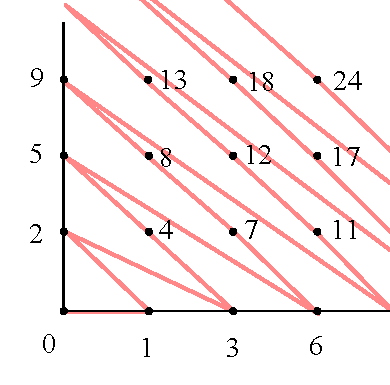
\includegraphics[width=0.25\columnwidth,keepaspectratio]{dove-tail.pdf}
\end{figure}


\end{document}
